\documentclass[10pt,compress,usetitleprogressbar,mathserif]{beamer}
\usepackage[spanish, es-tabla,es-noquoting,es-noshorthands]{babel}
\usepackage{tikz}
\usepackage{showexpl}
\usepackage{amsthm}
\usepackage{amsmath}
\usepackage{amssymb}
\usepackage{graphicx}
\graphicspath{{img/}}
\usepackage{booktabs}% http://ctan.org/pkg/booktabs
% Solarized palette
\definecolor{solarizedBase03}{HTML}{002B36}
\definecolor{solarizedBase02}{HTML}{073642}
\definecolor{solarizedBase01}{HTML}{586e75}
\definecolor{solarizedBase00}{HTML}{657b83}
\definecolor{solarizedBase0}{HTML}{839496}
\definecolor{solarizedBase1}{HTML}{93a1a1}
\definecolor{solarizedBase2}{HTML}{EEE8D5}
\definecolor{solarizedBase3}{HTML}{FDF6E3}
\definecolor{solarizedYellow}{HTML}{B58900}
\definecolor{solarizedOrange}{HTML}{CB4B16}
\definecolor{solarizedRed}{HTML}{DC322F}
\definecolor{solarizedMagenta}{HTML}{D33682}
\definecolor{solarizedViolet}{HTML}{6C71C4}
\definecolor{solarizedBlue}{HTML}{268BD2}
\definecolor{solarizedCyan}{HTML}{2AA198}
\definecolor{solarizedGreen}{HTML}{859900}

\setbeamercovered{dynamic}

\usetheme{epstfg}
\setbeamertemplate{note page}[compress]
\title{Práctica 1}
\author{Pablo Baeyens \and Antonio Checa \and Iñaki Madinabeitia \and José Manuel Muñoz \and Darío Sierra}
\date{Algorítmica}
\def\inline{\lstinline[basicstyle=\ttfamily]}

\begin{document}
\maketitle

\begin{frame}{Índice}
  \tableofcontents
\end{frame}

\section{Ejercicio 1: \large{Eficiencia Empírica }}

\subsection{Algoritmos Cuadráticos}

\begin{frame}{Burbuja}
	\resizebox{\linewidth}{!}{
	\hspace{1cm}
	\begin{tabular}{l ||*{7}{c}}
	%	\hline
	Datos & 2000 & 4000 & 6000 & 8000 & 10000 & 12000 & 14000 \\
	Tiempo (s) & 0.0140894 & 0.0515536 & 0.113751 & 0.202951 & 0.317834 & 0.467509 & 0.637843	\\
	\hline
	Datos  & 16000 & 18000 & 20000 & 22000 & 24000 & 26000 & 28000 \\
	Tiempo (s) & 0.831875 & 1.05149 & 1.2976 & 1.56672 & 1.85661 & 2.1866 & 2.52668	\\
	\hline
	Datos & 30000 & 32000 & 34000 & 36000 & 38000 & 40000 & 42000 \\
	Tiempo (s)& 2.90867 & 3.32019 & 3.72809 & 4.19815 & 4.67249 & 5.15041 & 5.69877		\\
	\hline
	Datos & 44000 & 46000 & 48000 & 50000 \\
	Tiempo (s) & 6.25114 & 6.82935 & 7.43045 & 8.08572\\

	\end{tabular}
}
\end{frame}

\begin{frame}{Selección}
		\resizebox{\linewidth}{!}{
			\hspace{1cm}
			\begin{tabular}{l ||*{7}{c}}
				%	\hline
				Datos & 2000 & 4000 & 6000 & 8000 & 10000 & 12000 & 14000 \\
				Tiempo (s) & 0.0056981 & 0.0229513 & 0.0484921 & 0.085303 & 0.133457 & 0.192178 & 0.260748	\\
				\hline
				Datos  & 16000 & 18000 & 20000 & 22000 & 24000 & 26000 & 28000 \\
				Tiempo (s) & 0.344565 & 0.436515 & 0.532265 & 0.647896 & 0.765415 & 0.902801 & 1.04346	\\
				\hline
				Datos & 30000 & 32000 & 34000 & 36000 & 38000 & 40000 & 42000 \\
				Tiempo (s)& 1.20025 & 1.36391 & 1.5385 & 1.72302 & 1.91741 & 2.12458 & 2.34051		\\
				\hline
				Datos & 44000 & 46000 & 48000 & 50000 \\
				Tiempo (s) & 2.56741 & 2.80465 & 3.05395 & 3.3125\\

			\end{tabular}
		}

\end{frame}

\begin{frame}{Inserción}
		\resizebox{\linewidth}{!}{
			\hspace{1cm}
			\begin{tabular}{l ||*{7}{c}}
				%	\hline
				Datos & 2000 & 4000 & 6000 & 8000 & 10000 & 12000 & 14000 \\
				Tiempo (s) & 0.00500529 & 0.0211343 & 0.0423133 & 0.0749079 & 0.119386 & 0.171897 & 0.230161	\\
				\hline
				Datos  & 16000 & 18000 & 20000 & 22000 & 24000 & 26000 & 28000 \\
				Tiempo (s) & 0.306819 & 0.394836 & 0.471464 & 0.575623 & 0.669068 & 0.816444 & 0.915119	\\
				\hline
				Datos & 30000 & 32000 & 34000 & 36000 & 38000 & 40000 & 42000 \\
				Tiempo (s)  & 1.05814 & 1.19949 & 1.35952 & 1.51431 & 1.68403 & 1.88228 & 2.09879		\\
				\hline
				Datos & 44000 & 46000 & 48000 & 50000 \\
				Tiempo (s) & 2.26926 & 2.46238 & 2.66613 & 2.92835\\

			\end{tabular}
		}
\end{frame}

\subsection{Algoritmos Cúbicos}

\begin{frame}{Algoritmo de Floyd}
	\resizebox{\linewidth}{!}{
		\hspace{1cm}
		\begin{tabular}{l ||*{7}{c}}
			%	\hline
				Datos & 30 & 60 & 90 & 120 & 150 & 180 & 210 \\
				Tiempo (s) & 0.000280424 & 0.00160165 & 0.00577986 & 0.0112503 & 0.0211072 & 0.0354685 & 0.0557242	\\
				\hline
				Datos  & 240 & 270 & 300 & 330 & 360 & 390 & 420 \\
				Tiempo (s) & 0.0824679 & 0.119058 & 0.160319 & 0.213182 & 0.281825 & 0.358154	\\
				\hline
				Datos & 450 & 480 & 510 & 540 & 570 & 600 & 630 \\
				Tiempo (s) & 0.543534 & 0.6525 & 0.790683 & 0.929593 & 1.09787 & 1.27982 & 1.47915	\\
				\hline
				Datos & 660 & 690 & 720 & 750 \\
				Tiempo (s) & 1.70325 &1.94156& 2.19971 &2.48584\\

		\end{tabular}
	}
\end{frame}

\subsection{Algoritmos $n\cdot log(n)$ }

\begin{frame}{Quicksort}
	\resizebox{\linewidth}{!}{
		\hspace{1cm}
		\begin{tabular}{l ||*{7}{c}}
			%	\hline
			Datos & 2000 & 4000 & 6000 & 8000 & 10000 & 12000 & 14000 \\
			Tiempo (s) & 0.000255184 & 0.000380688 & 0.000627165 & 0.000811187 & 0.00115236 & 0.00135381 & 0.00151702	\\
			\hline
			Datos  & 16000 & 18000 & 20000 & 22000 & 24000 & 26000 & 28000 \\
			Tiempo (s) & 0.00176841  & 0.00198622 & 0.00230529 & 0.00243562 & 0.00272028 & 0.0029159 & 0.00333496	\\
			\hline
			Datos & 30000 & 32000 & 34000 & 36000 & 38000 & 40000 & 42000 \\
			Tiempo (s)& 	0.00344278 & 0.00368476 & 0.00396666 & 0.00417767 & 0.00435608 & 0.00471517 & 0.00485819	\\
			\hline
			Datos & 44000 & 46000 & 48000 & 50000 \\
			Tiempo (s) & 0.00518884 & 0.00542106 & 0.00569736 & 0.00593068\\

		\end{tabular}
	}
\end{frame}

\begin{frame}{Heapsort}
		\resizebox{\linewidth}{!}{
			\hspace{1cm}
			\begin{tabular}{l ||*{7}{c}}
				%	\hline
				Datos & 2000 & 4000 & 6000 & 8000 & 10000 & 12000 & 14000 \\
				Tiempo (s) & 0.000235276 & 0.00050898 & 0.000883159 & 0.0011282 & 0.00141654 & 0.00181285 & 0.0021804	\\
				\hline
				Datos  & 16000 & 18000 & 20000 & 22000 & 24000 & 26000 & 28000 \\
				Tiempo (s) & 0.0024347 & 0.00273261 & 0.00328375 & 0.0034868 & 0.00374075 & 0.00421249 & 0.00447123	\\
				\hline
				Datos & 30000 & 32000 & 34000 & 36000 & 38000 & 40000 & 42000\\
				Tiempo (s)& 	0.00478116 & 0.00530559 & 0.00550902 & 0.00590121 & 0.0061024 & 0.00662012 & 0.00693612	\\
				\hline
				Datos & 44000 & 46000 & 48000 & 50000 \\
				Tiempo (s) & 0.00733094 & 0.00750173 & 0.00784107 & 0.00840717\\

			\end{tabular}
		}
\end{frame}

\begin{frame}{Mergesort}
		\resizebox{\linewidth}{!}{
			\hspace{1cm}
			\begin{tabular}{l ||*{7}{c}}
				%	\hline
				Datos & 2000 & 4000 & 6000 & 8000 & 10000 & 12000 & 14000 \\
				Tiempo (s) & 0.000271712 & 0.000580481 & 0.00110623 & 0.00136628 & 0.00175957 & 0.00236303 & 0.00228759	\\
				\hline
				Datos  & 16000 & 18000 & 20000 & 22000 & 24000 & 26000 & 28000 \\
				Tiempo (s) & 0.00264795 & 0.00315738 & 0.00382311 & 0.00425249 & 0.00498035 & 0.00438116 & 0.00489393	\\
				\hline
				Datos & 30000 & 32000 & 34000 & 36000 & 38000 & 40000 & 42000 \\
				Tiempo (s)& 0.00515919 & 0.00553019 & 0.00621929 & 0.00660115 & 0.00701515 & 0.00753488 & 0.00811711		\\
				\hline
				Datos & 44000 & 46000 & 48000 & 50000 \\
				Tiempo (s)  & 0.00946593 & 0.00930644 & 0.00988324 & 0.0106572\\

			\end{tabular}
		}
\end{frame}
\subsection{Algoritmos exponenciales}

\begin{frame}{Fibonacci $t_n=t_{n-1}+t_{n-2}$}
		\resizebox{\linewidth}{!}{
			\hspace{1cm}
			\begin{tabular}{l ||*{7}{c}}
				%	\hline
				Datos &1 & 2 & 3 & 4 & 5 & 6 & 7  \\
				Tiempo (s) & 1.79e-07 & 1.88e-07 & 2.05e-07 &  2.89e-07  & 2.61e-07 & 2.87e-07 & 4.65e-07	\\
				\hline
				Datos & 8 & 9 & 10 & 11& 12 & 13 & 14 \\
				Tiempo (s) & 7.53e-07 & 1.131e-06 & 1.365e-06 & 1.796e-06 & 1.671e-06 & 3.612e-06 & 7.294e-06	\\
				\hline
				Datos & 15 & 16 & 17 & 18 & 19 & 20 & 21 \\
				Tiempo (s)& 	7.834e-06 & 1.2102e-05 & 1.7977e-05 & 2.9478e-05 & 5.3614e-05 & 7.2343e-05 & 0.000132759	\\
				\hline
				Datos & 22 & 23 & 24 & 25 \\
				Tiempo (s) & 0.000189094 & 0.000315282 & 0.000499445 &  0.000675111\\

			\end{tabular}
		}
\end{frame}

\begin{frame}{Hanói $t_n=2 \cdot t_{n-1}+1 $}
		\resizebox{\linewidth}{!}{
			\hspace{1cm}

			\begin{tabular}{l ||*{7}{c}}
				%	\hline
				Datos &1 & 2 & 3 & 4 & 5 & 6 & 7  \\
				Tiempo (s) & 1.85e-07 & 2.52e-07 & 3.63e-07 & 5.65e-07 & 5.96e-07 &  1.206e-06 & 1.909e-06	\\
				\hline
				Datos & 8 & 9 & 10 & 11& 12 & 13 & 14 \\
				Tiempo (s) & 3.047e-06 & 5.639e-06 & 1.1064e-05 & 2.1002e-05 & 3.7705e-05 & 7.8102e-05 & 0.000165379	\\
				\hline
				Datos & 15 & 16 & 17 & 18 & 19 & 20 & 21 \\
				Tiempo (s)& 	0.000334135 & 0.000589484 & 0.000988963 & 0.0017404 & 0.00368885 & 0.00684205 & 0.0136331	\\
				\hline
				Datos & 22 & 23 & 24 & 25 \\
				Tiempo (s) & 0.0273772 & 0.05418 & 0.107202 & 0.214262\\

			\end{tabular}
		}
\end{frame}

\section{Ejercicio 2: \large{Elaboración de Gráficas}}

\begin{frame}{Burbuja}
	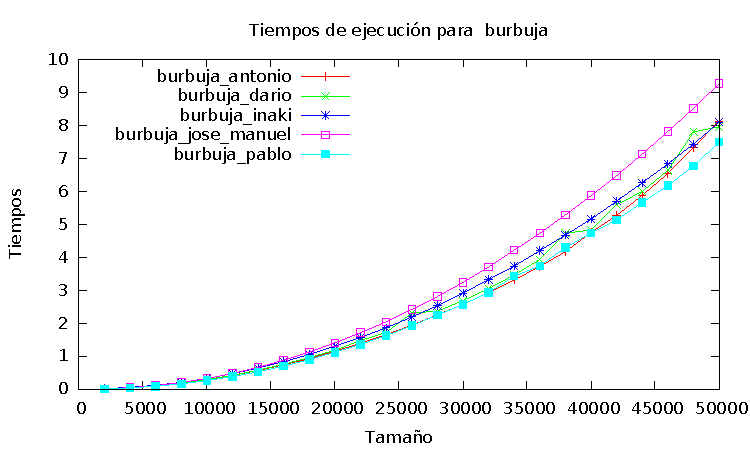
\includegraphics[width = \textwidth ]{burbuja_todos_g}
\end{frame}

\begin{frame}{Selección}
	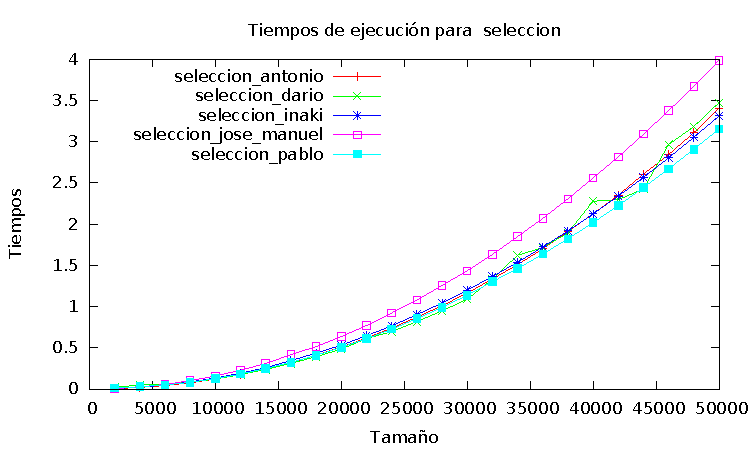
\includegraphics[width = \textwidth ]{seleccion_todos_g}
\end{frame}

\begin{frame}{Inserción}
	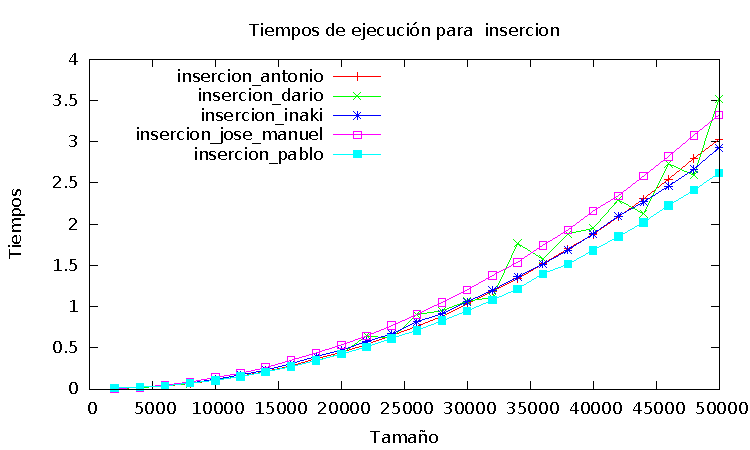
\includegraphics[width = \textwidth ]{insercion_todos_g}
\end{frame}

\begin{frame}{Comparativa: Algoritmos Cuadráticos}
	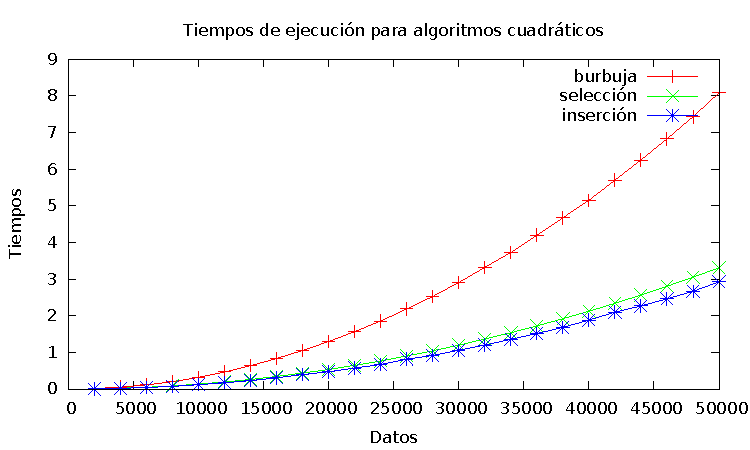
\includegraphics[width = \textwidth ]{comparativa_cuadraticos_g}
\end{frame}

\begin{frame}{Mergesort}
	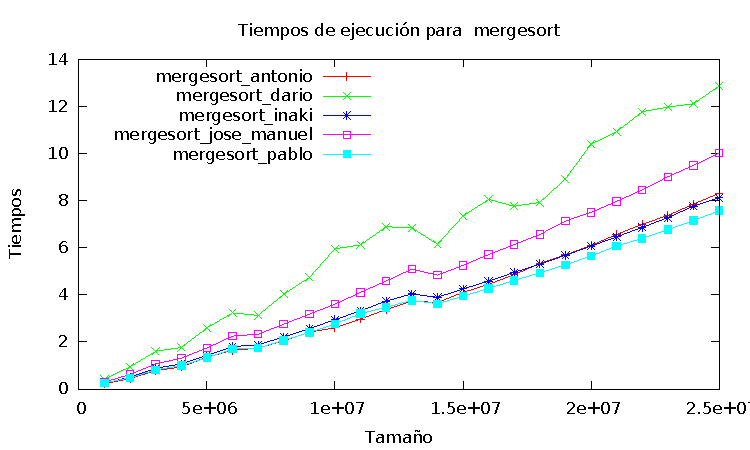
\includegraphics[width = \textwidth ]{mergesort_todos_g}
\end{frame}

\begin{frame}{Quicksort}
	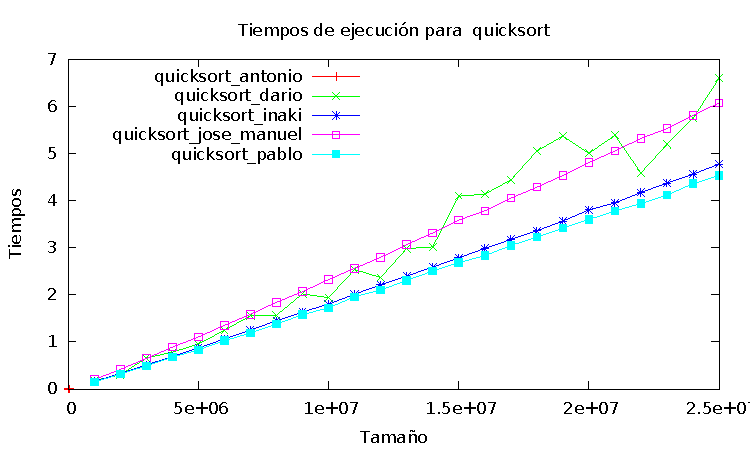
\includegraphics[width = \textwidth ]{quicksort_todos_g}
\end{frame}

\begin{frame}{Heapsort}
	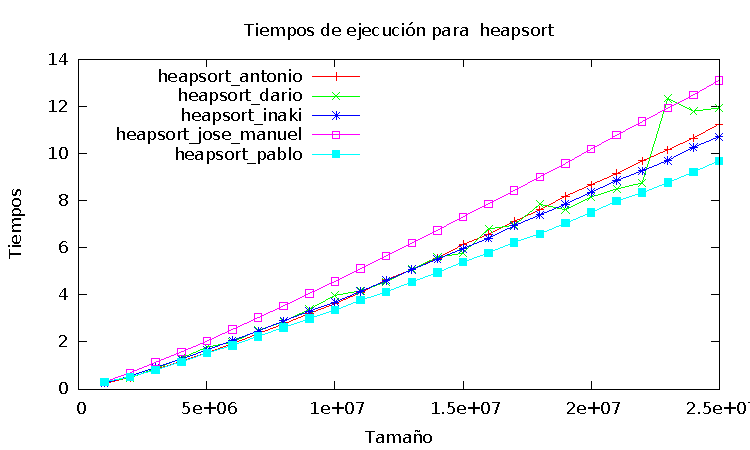
\includegraphics[width = \textwidth ]{heapsort_todos_g}
\end{frame}

\begin{frame}{Comparativa: Algoritmos O$(nlog(n))$}
		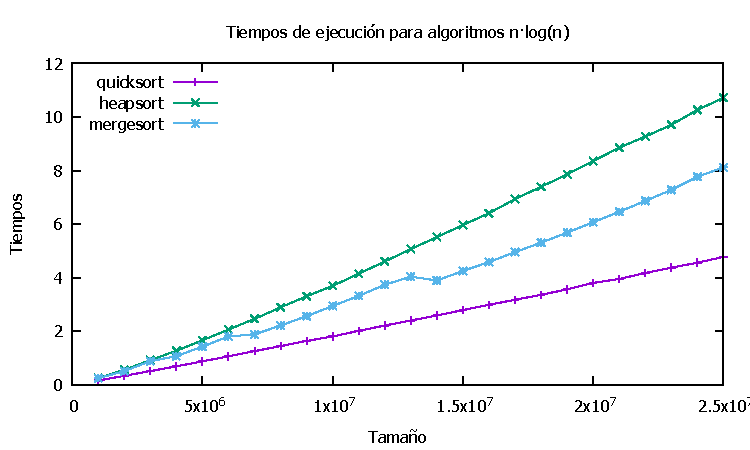
\includegraphics[width = \textwidth ]{comparativa_logaritmicos_g}
\end{frame}

\begin{frame}{Algoritmo de Floyd}
		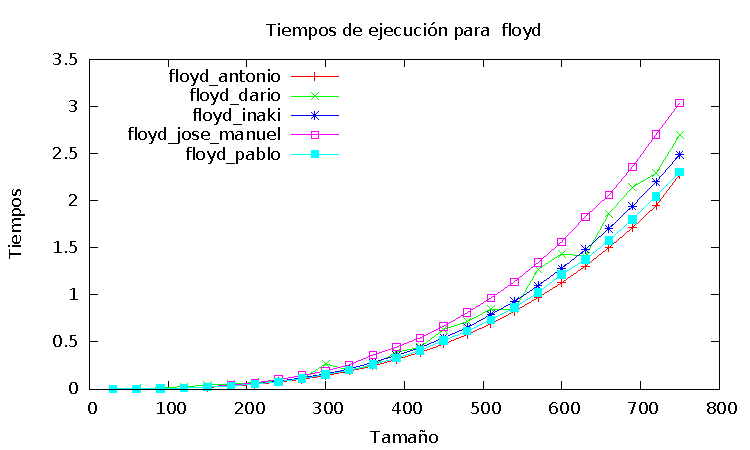
\includegraphics[width = \textwidth ]{floyd_todos_g}
\end{frame}

\begin{frame}{Fibonacci}
		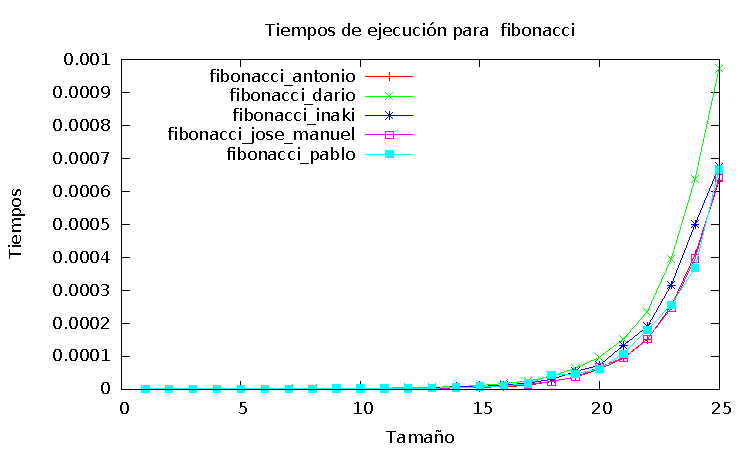
\includegraphics[width = \textwidth ]{fibonacci_todos_g}
\end{frame}

\begin{frame}{Hanói}
		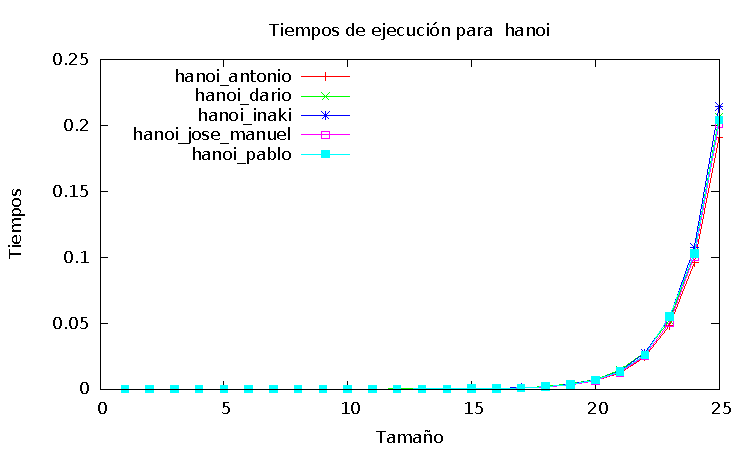
\includegraphics[width = \textwidth ]{hanoi_todos_g}
\end{frame}

\begin{frame}{Comparativa global de los algoritmos}
		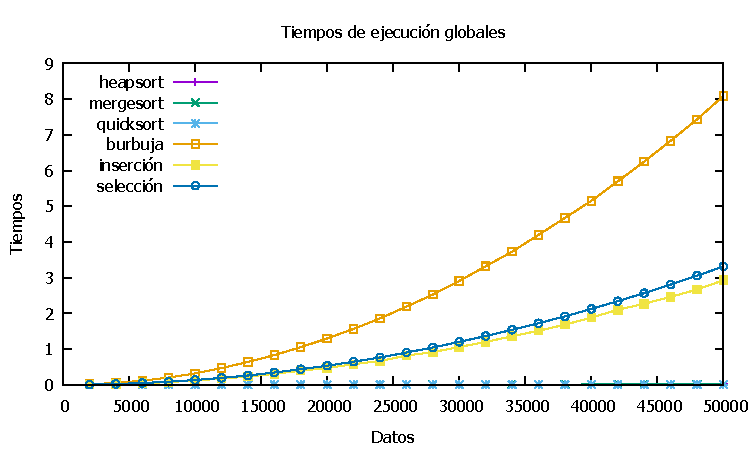
\includegraphics[width = \textwidth ]{comparativa_global_g}
\end{frame}


\end{document}
